% We extend the work of \citet{busse2017double} by including the two factors of \citet{FAMA20151} to their double-adjusted performance measure. Specifically, we compute risk-adjusted returns (alphas) from the \citet{carhart1997persistence} four-factor model and from a six-factor model including the profitability and investment factors. We conduct cross-sectional regressions of mutual fund alphas on fund-level characteristics, and use the cross-sectional estimates to decompose alpha into double-adjusted alpha and characteristics-driven performance. We also use simulations ... 
% \subsection{Double-adjusted performance measures}
\label{section4}

% This section describes our new mutual fund performance measure which adjusts fund returns for both factor betas and characteristics. Section \ref{double_alpha} discusses the model used to obtain the double-adjusted performance measure. Section \ref{Bayes_Model} describes the Bayesian techniques used to estimate the model. Section \ref{estimation_results} discusses the main results from the model estimation.

There are many alternatives to evaluate the performance of mutual funds. A common performance measure is a fund's alpha, the return adjusted for exposures to risk factors that drives most of the fund's return. The intercept (alpha) is then interpreted as the abnormal return reflecting the ability of the fund manager. Alternatively, funds are evaluated relative to the characteristic-based benchmark approach of Daniel, Grinblatt, Titman, and Wermers (DGTW; 1997). The DGTW measure controls for the main anomalies through characteristic-sorted portfolio returns. We will examine this measure in Section \ref{section5B}. 

% \par \citet{brennan1998alternative} was the first to look beyond a unilateral explanation of cross-sectional variation in expected returns by either factor betas or characteristics. They first estimate alpha from a factor model. Using the resulting estimates of alpha they run the following cross-sectional regressions 
% \begin{equation}
%     \label{double}
%     \alpha_{it} = \delta_{0t} + \delta_{1t}'Z_{it-1} + \eta_{it},
% \end{equation}
% where $\alpha_{it}$ is the standard factor model alpha of stock $i$ estimated with returns up until time $t$ and $Z_{it-1}$ are lagged  characteristics. They find that characteristics (e.g., size, book-to-market, momentum) remain significantly related to expected returns even after the risk-adjustment by a factor model with risk factors based on those same characteristics. However, the dependent variable in Eq.(\ref{double})
% is estimated (with error) from a factor model as we can not observe the true alpha. 
% \footnote{As an alternative to the cross-sectional regression approach, \citet{busse2017double} propose a second approach to calculate their double-adjusted performance measure. In particular, they assign funds into portfolios based on a three-way sort on fund-level characteristics, and compare a fund's alpha to the average alpha of the characteristic-based portfolio to which the fund is assigned to. They find that using the portfolio-sorting approach does not materially differ the results.} Through simulations they show that their double-adjusted measure is less prone to erroneous indication of skill, thus being a better indication of managerial skill. 

We develop a performance measure which adjusts the alphas from a linear factor model for fund exposures to characteristics. We adopt a system of equations in which we simultaneously model conditional factor model alphas and analyze the cross-sectional relation between fund alphas and characteristics. The model takes on the following structure:   
\begin{alignat}{2}
    \label{asset}
    R_{i\tau,t} &= \alpha_{it} + \beta_{it}'F_{\tau,t} + \epsilon_{i\tau,t}, \hspace{0.2cm} \epsilon_{i\tau,t} \sim \mathcal{N}(0,\sigma^2_{\epsilon_{it}}), \hspace{0.1cm} \tau = t-\mathcal{T}+1,...,t,  
\hspace{0.1cm} i = 1,...,N_t \\
    \label{cross}
    \alpha_{it} &= \delta_{0t} + \delta_{1t}'Z_{it-1} + \eta_{it}, \hspace{0.2cm} \eta_{it} \sim \mathcal{N}(0,\sigma^2_{\eta t}), \hspace{0.1cm} t = 1,...,T,
\end{alignat}
where $R_{i\tau,t}$ and $F_{\tau,t}$ are daily excess returns of fund $i$ and daily factor returns, respectively. The superscript $\tau$ is used to index the daily returns in the rolling window ending in month $t$ and $\mathcal{T}$ is the length of the rolling window, that is, two years ($\mathcal{T}$ $\approx$ 500 trading days). 

The vector $\delta_t$ = [$\delta_{0t}$ $\delta_{1t}$]' contains the coefficients that measures for a given month $t$  the average abnormal returns of mutual funds and the relation between alphas ($\alpha_{it}$) and characteristics ($Z_{it-1}$). We follow \citet{cederburg2015asset} in adding a third layer to the model hierarchy:\footnote{\citet{cederburg2015asset} propose a hierarchical Bayes approach to model CAPM alphas conditioned on a set of firm characteristics. Our model extends their work by including daily returns and by evaluating a larger set of risk factors. Another example of hierarchical Bayes is presented in \citet{cosemans2015estimating}, which specify a hierarchical prior on the parameters in their conditional factor beta model. } 
\begin{equation}
\label{delta_t}
\delta_t = \bar{\delta} + v_t, \hspace{0.2cm} v_t \sim \mathcal{N}(0,\Sigma_{\delta}), \hspace{0.1cm} t = 1,...,T,
\end{equation}
where the monthly coefficients $\{\delta_t\}^T_{t=1}$ are drawn from a multivariate normal distribution centered at $\bar{\delta}$ with covariance matrix $\Sigma_\delta$. This layer of the model means that the coefficients $\delta_t$ can be interpreted as time-random effects in a panel-data model.

We treat $\bar{\delta}$ as an unknown parameter and aggregate the evidence about $\delta_t$ across each month in our sample to estimate $\bar{\delta}$. If the factor model prices the mutual funds, we should not find a significant (systematic) relation between alphas and characteristics, such that the elements of $\bar{\delta}$ should be centered around zero. If an element of $\bar{\delta}$ deviates from zero, there is evidence that the factor model inadequately adjusts for exposure to a certain characteristic, such that fund managers can generate alpha by passively loading on this characteristic. In the remainder of this paper, we analyze $\bar{\delta}$ when assessing the importance of adjusting alpha for passive exposures to characteristics.

Eq.(\ref{asset}) represents the factor model for each fund $i$ based on daily fund returns from the rolling window. In our empirical analysis we use a six-factor model which augments the \citet{carhart1997persistence} four-factor model with the profitability and investment factors from \citet{FAMA20151}.
In Eq.(\ref{cross}), we relate the cross-section of alphas to the  characteristics from the previous month. In $Z$ we include the logarithm of market capitalization (Mcap), the logarithm of book-to-market ratio (B/M), the logarithm of one plus the past twelve-month cumulative return (Mom12), operating profitability (Profit), and asset growth (Invest). Before including them in the regressions, each characteristic is standardized by subtracting the cross-sectional mean in each month. In each rolling window we obtain estimates of $\alpha_{it}$ and $\delta_t$ and we roll the window a month at a time. 

Using the definitions in \citet{busse2017double}, double-adjusted performance measure of fund $i$ in month $t$ is defined as 
\begin{equation}
\label{double_adjusted_alpha}
     \alpha^*_{it} = \alpha_{it} - \delta_{1t}'Z_{it-1} = \delta_{0t} + \eta_{it}. 
\end{equation}
In this way we control for both the exposures to risk factors through $\alpha_{it}$ and the effects of firm characteristics by subtracting the component of alpha attributable to passive exposures to firm characteristics. Characteristic-driven performance is defined as
\begin{equation}
\label{char}
    \alpha^{char}_{it} = \alpha_{it} - \alpha^*_{it} = \delta_{1t}'Z_{it-1}.
\end{equation}

The errors in Eqs.(\ref{asset}) and (\ref{cross}) are assumed to be independent and normally distributed, such that excess returns are conditionally independent across funds and within rolling windows. Similarly, alphas are conditionally independent across funds and the monthly relations $\delta_t$ are independent conditional on $\bar{\delta}$. The main advantage of the specification of independent errors in returns and alphas is that we avoid the estimation of large variance-covariance matrices to capture autocorrelations and cross-sectional correlations.

\subsection{Model Estimation}
\label{Bayes_Model} 
We adopt a hierarchical Bayes approach to estimate Eqs.(\ref{asset}), (\ref{cross}) and (\ref{delta_t}) simultaneously.\footnote{The first examples of Bayesian inference in asset pricing models are presented in \citet{mcculloch1990posterior} and \citet{harvey1990bayesian}. More recently, \citet{cremers2006multifactor} propose Bayesian tests for the mean-variance efficiency of a given portfolio. \citet{avramov2006exact} tests the international Capital Asset Pricing Model (ICAPM) with time-varying risk premia using posterior probabilities.} This approach yields several advantages over the alternatives, as the Bayesian approach is computationally more attractive than maximum likelihood estimation, and yields better finite sample properties than General Method of Moments (GMM).\footnote{\citet{ferson1995method} demonstrate that GMM has poor finite sample properties in the context of latent variable asset pricing models.} 
% \citet{cosemans2015estimating} propose a hybrid approach for estimating market beta by shrinking rolling window estimates toward a firm-specific prior motivated by economic theory.
 Another main advantage of our model is that we estimate all model parameters simultaneously. Conversely, a majority of previous studies employ a two-pass procedure to estimate the relation between alphas and characteristics (e.g., \citet{brennan1998alternative}, \citet{avramov2006asset} and \citet{busse2017double}). \citet{brennan1998alternative} find that characteristics (e.g., size, book-to-market, momentum) remain significantly related to expected returns even after the risk-adjustment by a factor model with risk factors based on those same characteristics. The two-step procedure includes the estimation of a factor model before regressing the resulting estimates of alpha on the firm characteristics. In the first step alphas are estimated with error such that the variance of these estimates equal the variance of the true alphas plus a measurement error term. Consequently, the standard errors of the estimated coefficients in the second-step regression are overstated. This measurement error may lead to insignificant coefficients even if the data conveys a significant relation between alphas and characteristics. A simultaneous estimation of all model parameters mitigates this measurement error problem.


% We estimate the panel model in Eq.(\ref{double_alpha}) using a flexible Bayesian method that yields a better bias-variance trade-off than standard frequentist methods. In particular, the Bayesian estimation increases precision by estimating the factor model using panel data, imposing a common structure on the factor betas while still allowing for cross-sectional heterogeneity. The advantage of this approach stems in part from the additional data used to estimate the factor model, which is useful given the monthly frequency of our data. In addition, by pooling the $\alpha_1$ loadings on characteristics, we exploit cross-sectional information to obtain more precise estimates, while we let the constant $\alpha_{0i}$ vary across funds to mitigate estimation bias. The traditional method for estimating conditional alphas, that is, running a separate OLS regression for each fund, also allows for cross-sectional heterogeneity but leads to large measurement errors because it does not exploit cross-sectional information.\footnote{We refer to  \citet{christopherson1999performance} and \citet{ferson2008asset} for an extensive reading on the estimation of conditional alphas, the implications of conditional alphas for the empirical asset pricing, and the main pitfalls. } The other extreme is to estimate conditional alphas in a pooled OLS regression, which leads to precise, but biased, estimates because it does not capture unobserved cross-sectional heterogeneity in the parameters.

\subsubsection{ Prior Distributions}
\label{priors}
To conduct Bayesian estimation techniques, we need to specify prior distributions for the model parameters. A prior distribution incorporates a researcher's belief about the parameter of interest, often founded on empirical research or economic theory. We specify proper, but relatively uninformative, priors for all parameters.\footnote{\citet{hobert1996effect} advocate the use of proper priors in estimating hierarchical models. They find that using improper priors may lead to improper posterior distributions which is difficult to detect from posterior draws.}
\par Regarding the loadings on characteristics, the expression in Eq.(\ref{delta_t}) implies the following hierarchical prior on $\delta_t$  
\begin{equation}
    \delta_t|\bar{\delta},\Sigma_\delta \sim \mathcal{N}(\bar{\delta},\Sigma_\delta), 
\end{equation}
which is a normal distribution with location parameter $\bar{\delta}$ and covariance matrix $\Sigma_\delta$. We treat $\bar{\delta}$ and $\Sigma_\delta$ as unknown parameters and assume the following uninformative priors 
\begin{equation}
    \bar{\delta} \sim \mathcal{N}\left(d, \Sigma_{d}\right),
\end{equation}
\begin{equation}
    \Sigma_\delta \sim IW\left([\psi_{\delta}S_\delta],\psi_{\delta}\right),
\end{equation}
where $IW$ denotes the inverted Wishart distribution with degrees of freedom $\psi_{\delta}$ and scale matrix $[\psi_{\delta}S_{\delta}]$.  We specify an uninformative prior for $\bar{\delta}$ by setting $d$ equal to the zero vector and $\Sigma_d$ to 100$I$, where $I$ is the identity matrix. Setting $d$ equal to the zero vector implies that alphas are not associated with characteristics, which contradicts previous empirical findings. However, by setting the diagonal elements of $\Sigma_d$ to large values we minimize the influence of the prior on the posterior distribution of $\bar{\delta}$. $\psi_{\beta}$ is set to the dimension of $\Sigma_{\delta}$, since this value gives the lowest weight to the prior (see, \citet{gelman2014bayesian}). The matrix $S_{\delta}$ is the prior mean of $\Sigma_{\delta}$ and is set to $I$. 
\par Regarding the fund-specific parameters, the hierarchical structure of our model implies the following prior on $\alpha_{it}$
\begin{equation}
    \alpha_{it}| \delta_t,\sigma^2_{\eta t} \sim \mathcal{N}(\delta_{0t}+\delta_{1t}'Z_{it-1},\sigma^2_{\eta t}), 
\end{equation}
in which the prior mean is dependent on characteristics. The posterior of $\alpha_{it}$ combines information from both the fund-specific time series of returns and from the cross-section of alphas. The relative importance of both components depends on the rolling window size $\mathcal{T}$ and the cross-sectional residual variance $\sigma^2_{\eta t}$. We specify a conjugate prior for $\beta_{it}$ as 
\begin{equation}
    \beta_{it} \sim \mathcal{N}(\bar{\beta},\Sigma_{\beta}), 
\end{equation}
where we set $\bar{\beta}$ equal to the sample mean of rolling window estimates of fund betas (see Panel D of Table 1). We define $\Sigma_\beta$ equal to 10$I$ to let the data speak for itself.
\par We complete the prior specification of our model by specifying conjugate priors for the idiosyncratic variances $\sigma^2_{\epsilon_{it}}$ and $\sigma^2_{\eta t}$ as
\begin{equation}
    \sigma^2_{\epsilon_{it}} \sim IG2(v_{\epsilon},s_\epsilon)  
\end{equation}
\begin{equation}
    \sigma^2_{\eta t} \sim IG2(v_{\eta},s_\eta), 
\end{equation}
where $IG2$ denotes the inverted Gamma-2 distribution. We specify relative uninformative priors by setting the degrees of freedom parameters $v_{\epsilon}$ and $v_{\eta}$ equal to 3 and the scale parameters $s_{\epsilon}$ and $s_{\eta}$ equal to $10^{-3}$. 

% We follow \citet{pastor2002investing} by setting $\bar{\alpha}_{0i}$ equal to -1 multiplied by the annual expense ratio divided by 12. Intuitively, we center the prior at a belief that fund managers possess no skill and that investing in mutual funds will under perform the benchmark by the fund's expenses.\footnote{The added value of actively managed mutual funds is an enduring topic within financial economics. The general consensus emanating across researchers is that fund managerial skill exists, but dissipated by increasing fund fees. An influential paper was \citet{fama2010luck}, which find evidence of superior performance among a small group of funds when analyzing gross returns, but these patters are masked when net returns are used. \citet{barras2010false} find that about one fifth of the funds truly yields negative alpha, while they find a small proportion of funds with truly positive performance, which are concentrated in the extreme right tail of the alpha distribution. } Setting the prior variance $\sigma^2_{\alpha_{0i}}$ equal to zero implies no prior belief in fund managerial skill and is equivalent to setting $\alpha_{0i}$ equal to $\bar{\alpha}_{0i}$. Conversely, setting $\sigma^2_{\alpha_{0i}}$ = $\infty$ is a diffuse prior which allows the data to dominate the posterior estimate. We set $\sigma^2_{\alpha_{0i}}$ to 0.1, which is a relatively diffuse prior to let the data speak for itself.  
% \par For the remaining parameters we specify uninformative (diffuse) priors to minimize their influence on the posterior densities. For the pooled parameters $\alpha_1$, we specify the following prior distribution 
% \begin{equation}
%     \alpha_1 \sim \mathcal{N}\left(\bar{\alpha}_1,\Sigma_{\alpha_1}\right).
% \end{equation}
% We specify an uninformative prior by setting the location parameter $\bar{\alpha}_1$ equal to the zero vector and $\Sigma_{\alpha_1}$ to 100$I$, with $I$ denoting the identity matrix. We specify a diffuse prior for the idiosyncratic volatility $\sigma^2_{\eta_i}$: 
% \begin{equation}
%     p(\sigma^2) \propto \frac{1}{\sigma^2_{\eta_i}}. 
% \end{equation}
% \par To complete the prior specification of the model, we set a hierarchical prior for the factor betas. Particularly, we specify a common prior for $\beta_i$: 
% \begin{equation}
%     \beta_i \sim \mathcal{N}\left(\bar{\beta},\Sigma_{\beta}\right), 
% \end{equation} 
% which imposes a common structure on the posterior estimates of $\beta_i$ across funds, while still allowing for cross-sectional heterogeneity. Intuitively, imposing a very sharp prior on $\beta_i$ by setting the diagonal elements of the covariance matrix $\Sigma_{\beta}$ equal to small values is equivalent to pooling the factor betas across funds. Conversely, if we specify an uninformative prior by setting the diagonal elements of $\Sigma_{\beta}$ to large values we are practically running separate OLS regressions for each individual fund. 
% \par We follow \citet{cosemans2015estimating} in treating the prior moments as random variables and assume the following diffuse priors for these parameters 
% \begin{equation}
%     \bar{\beta} \sim \mathcal{N}\left(b,\Sigma_b\right), 
% \end{equation}
% \begin{equation}
%     \Sigma_\beta \sim IW\left([\psi_{\beta}S_\beta],\psi_{\beta}\right),
% \end{equation}
% where $IW$ denotes the inverted Wishart distribution with degrees of freedom $\psi_{\beta}$ and scale matrix $[\psi_{\beta}S_{\beta}]$. We specify an uninformative prior for $\bar{\beta}$ by setting $b$ equal to the zero vector and $\Sigma_{\beta}$ to 100$I$. $\psi_{\beta}$ is set to the dimension of $\Sigma_{\beta}$, since this value gives the lowest weight to the prior (see, Gelman et al. 2014). The matrix $S_{\beta}$ is the prior mean of $\Sigma_{\beta}$ and is set to $I$.

\subsubsection{Markov Chain Monte Carlo Gibbs Sampler}
We employ the Markov Chain Monte Carlo (MCMC) Gibbs sampler\footnote{For an extensive reading on the application of the Gibbs sampler in several econometric models, we refer to \citet{de2006gibbs}.} to estimate the model. An attractive feature of MCMC techniques is that samples of random drawings of the model parameters $\theta$ can be generated from the joint posterior indirectly, without the need to specify the exact form of this joint distribution directly. The Gibbs sampler uses an iterative procedure to create Markov chains by simulating from full conditional posteriors instead which are typically much easier to derive. In particular, the parameter vector $\theta$ is partitioned into $B$ blocks ($\theta^{(1)}$,...,$\theta^{(B)}$). At each iteration of the Gibbs sampler each block is sampled from its posterior distribution conditioned on the other blocks and the data. After the Markov chains have converged, the sets of draws that are obtained from the conditional posteriors can be effectively considered as samples from the joint posterior. We provide the steps in the Gibbs sampler and the derivation of the full conditional posterior distributions in Appendix D. 
% \par To initialize the Gibbs sampler, we require starting values for the model parameters. For the fund-specific parameters, we estimate Eq.(\ref{asset}) for each fund in each rolling window and use the estimates as starting values for $\alpha_{it}$ and $\beta_{it}$. Each month $t$, we regress the estimates of alpha on a constant and the lagged characteristics using the cross-section of funds. The resulting estimates are used as starting values for $\delta_t$. The starting values for $\sigma^2_{\epsilon_{it}}$ and $\sigma^2_{\eta t}$ are set to the sample residual variance estimator from the corresponding regressions. For the hyperparameters $\bar{\delta}$ and $\Sigma_\delta$, we set the starting values equal to the sample mean and covariance matrix of the estimates $\{\delta_t\}^T_{t=1}$, respectively. 
\par To check the convergence of the Gibbs sampler, we turn to standard diagnostics tests, including the partial means test of Geweke (1992) and the Gelman-Rubin statistic described in \citet{gelman2014bayesian}. Both tests indicate that the Markov Chains have converged after 2500 iterations. Therefore, in our empirical analysis we run 5000 iterations of the Gibbs sampler and discard the first 2500 iterations as burn-in period. The remaining draws are used to derive posterior results. The $m^{\text{th}}$ draw of double-adjusted alpha and characteristic-driven performance are given by 
\begin{equation}
\label{posterior}
    \alpha_{it}^*^{(m)} = \alpha^{(m)}_{it} - \delta_{1t}'^{(m)}Z_{it-1} 
\hspace{0.5cm} \text{and} \hspace{0.5cm}
    \alpha_{it}^{char}^{(m)} =  \delta_{1t}'^{(m)}Z_{it-1}
\end{equation}
The posterior mean of draws $\{\alpha_{it}^{*}^{(m)}\}^{5000}_{m = 2501}$ and $\{\alpha_{it}^{char}^{(m)}\}^{5000}_{m = 2501}$ constitute the final estimates of double-adjusted alpha and characteristic-driven performance, respectively. 

% The $m^{\text{th}}$ draw of double-adjusted alpha and characteristic-driven performance are given by 
% \begin{equation}
%     \alpha_{it}^*^{(m)} = \alpha^{(m)}_{it} - \delta_{1t}'^{(m)}Z_{it-1} 
% \hspace{0.5cm} \text{and} \hspace{0.5cm}
%     \alpha_{it}^{char}^{(m)} =  \delta_{1t}'^{(m)}Z_{it-1}
% \end{equation}
% The posterior mean of draws $\{\alpha_{it}^{*}^{(m)}\}^{5000}_{m = 2501}$ and $\{\alpha_{it}^{char}^{(m)}\}^{5000}_{m = 2501}$ constitute the final estimates of double-adjusted alpha and characteristic-driven performance, respectively. 

% \renewcommand\labelenumi{\theenumi:}
% \begin{algorithm}
% \caption{MCMC Gibbs sampler}\label{gibbs}
%  \textsc{Inputs}: \{\{\{$R_{i\tau,t}, Z_{it-1}, F_{\tau,t}\}_{i=1} ^{N_t}}\}_{\tau = t -\mathcal{T} +1}^{t}\}_{t=1}^{T}$ (data)\\
% \textsc{Outputs}: $\{\theta^{(m)}\}_{m=1}^{M}$ (approximate sample from the joint posterior)  \vspace{0.2cm} \hline 
%  \begin{minipage}{.92\linewidth}
%  \vspace{0.2cm}
% \begin{enumerate}
% \item Set starting values for model parameters: \\ $\theta^{(0)}$ =  $\{ \{\{\alpha_{it}^{(0)}, \beta_{it}^{(0)}, \sigma^2_{\epsilon_{it}}^{(0)}\}^{N_t}_{i=1}, \delta^{(0)}_{t}, \sigma^2_{\eta t}^{(0)}\}^{T}_{t=1}, \bar{\delta}^{(0)}, \Sigma^{(0)}_{\delta}\}$ and set $m$ to 0. 
% \item Update parameters given current draws $\theta^{(m)}$:
% \begin{enumerate}[label=(\roman*)]
%     \item Sample $\alpha_{it}^{(m+1)}$, $\beta_{it}^{(m+1)}$ $|$ $\sigma^2_{
%  \epsilon_{it}}^{(m)}$, $\delta_t^{(m)}$, 
%   $\sigma^2_{\eta t}^{(m)}$, \hspace{0.1} for $i$ = 1,...,$N_t$, $t$ = 1,...,$T$. 
%   \item Sample $\sigma^2_{\epsilon_{it}}^{(m+1)}$ $|$ $\alpha^{(m+1)}_{it}$, $\beta_{it}^{(m+1)}$, \hspace{0.1} for $i$ = 1,...,$N_t$, $t$ = 1,...,$T$. 
%     \item Sample $\delta_{t}^{(m+1)}$ $|$ $\{\alpha_{it}^{(m)}\}^{N_t}_{i=1}$, $\sigma^2_{\eta t}^{(m)}$, $\bar{\delta}^{(m)}$, $\Sigma_{\delta}^{(m)}$, \hspace{0.1} for $t$ = 1,...,$T$. 
%     \item Sample $\sigma^2_{\eta t}^{(m+1)}$ $|$ $\{\alpha_{it}^{(m+1)}\}^{N_t}_{i=1}$, $\delta^{(m+1)}_t$, \hspace{0.1} for $t$ = 1,...,$T$.
%     \item Sample $\bar{\delta}^{(m+1)}$ $|$ $\{\delta_t^{(m+1)}\}^{T}_{t=1}$, $\Sigma_{\delta}^{(m)}$. 
%     \item Sample $\Sigma_{\delta}^{(m+1)}$ $|$ $\{\delta_t^{(m+1)}\}^{T}_{t=1}$, $\bar{\delta}^{(m+1)}$. 
% \end{enumerate}
% \item Set $m$ = $m$ + 1, and go to step 2. 
% \end{enumerate} 
% \end{minipage}
% \end{algorithm}

\subsection{Estimation Results}
\label{estimation_results}
Table \ref{table3} summarizes the relation between six-factor alphas and fund-level characteristics. In Panel A, we report the posterior estimates of the distribution of $\bar{\delta}$, which measures the systematic relation between alphas and characteristics over the entire sample period. When we estimate the model for each characteristic in isolation, we find that market capitalization (Mcap) and book-to-market (B/M) are negatively associated with alpha, while momentum return (Mom12) and asset growth (Invest) are positively associated with alpha. Alphas are unrelated to the profitability characteristic. If the characteristics are correlated with each other and offer little unique information about alphas then studying each characteristic in isolation will overstate the failings of the factor model. If we specify alpha as a linear combination of all characteristics, Mcap, B/M, Mom12 and Invest remain significantly associated with alphas. The constant term in Table \ref{table3} measures the outperformance of the average mutual fund relative to the Fama-French benchmarks, which we refer to as the aggregate alpha. Over our sample period we find that the average mutual fund earns negative risk-adjusted returns. 

% \begin{singlespacing}
% \begin{table}[h!]
% \small
% \centering
% \setlength{\tabcolsep}{16.5pt}
% {\captionsetup{justification=centering,singlelinecheck=off}
% \caption{\bfseries Six-factor alpha vs. characteristics }}
% \caption*{This table presents the results of the estimation of the model in Eqs.(\ref{asset}), (\ref{cross}) and (\ref{delta_t}). We estimate this model in each month during the period February 2001 to December 2016, using an estimation period of two years to estimate the six-factor model in Eq.(\ref{asset}), rolling the window a month at a time.
%  The characteristics (Z) are the logarithm of market capitalization (Mcap), the logarithm of book-to-market ratio (B/M), the logarithm of one plus the past twelve-month cumulative return (Mom12), operating profitability (Profit) and asset growth (Invest). Each characteristic is standardized by subtracting the cross-sectional mean each month. We estimate the model for each characteristic in isolation and for all characteristics in a joint model. Panel A presents the posterior mean and standard deviation for the aggregate-level parameters in $\bar{\delta}$, based on the posterior distribution of the parameters constructed from 5000 iterations of the Gibbs sampler with the first 2500 iterations discarded as a burn-in period. Panel B presents \citet{fama1973risk} estimates
%  and \citet{fama1973risk} t-statistics with the \citet{newey1986simple} correction of 12 lags. In Panel A, estimates in bold font indicate that the 95\% credible interval of the posterior distribution does not include zero. In Panel B,  estimates in bold font indicate significance at the 5\% level.
% }
% {\captionsetup{justification=centering,singlelinecheck=off}

% \begin{tabular}{lrrrrrr}
% \hline
% \multicolumn{7}{l}{Panel A: Simultaneous Bayesian estimation}                                   \\ Cnst & -\textbf{0.003}  & -\textbf{0.003} & -\textbf{0.003}& -\textbf{0.003}&-\textbf{0.003} & -\textbf{0.002}\\ & (0.000) & (0.000) & (0.000) & (0.000) & (0.000) & (0.000) \\ 
% Mcap   & -\textbf{0.002}  &                 &                &        &                & \textbf{-0.002}         \\
%       & (0.000)  &                 &                &        &                & (0.000)          \\
% B/M    &         & \textbf{-0.003} &                &        &                & \textbf{-0.004} \\
%       &         & (0.000)          &                &        &                & (0.000)          \\
% Mom12  &         &                 & \textbf{0.019} &        &                & \textbf{0.005}  \\
%       &         &                 & (0.002)         &        &                & (0.003)          \\
% Profit &         &                 &                & -0.011  &                & -0.003         \\
%       &         &                 &                & (0.002) &                & (0.002)          \\
% Invest &         &                 &                &        & \textbf{0.024} & \textbf{0.017}  \\
%       &         &                 &                &        & (0.004)         & (0.004)          \\
%       &         &                 &                &        &                &                 \\
% \multicolumn{7}{l}{Panel B: Two-step OLS approach}                                   \\  Cnst & -0.002 & -0.002 &-0.002 & -0.002 & -0.002  & -0.002 \\ & (-1.40) & (-1.40) & (-1.40) & (-1.40) & (-1.40) & (-1.40) \\ 
% Mcap   & -0.001 &         &        &         &        & -0.002  \\
%       & (1.81) &         &        &         &        & (-1.60)  \\
% B/M    &        & \textbf{-0.005}  &        &         &        & \textbf{-0.006}  \\
%       &        & (-2.45) &        &         &        & (-2.29) \\
% Mom12  &        &         & \textbf{0.016}  &         &        & 0.002   \\
%       &        &         & (4.66) &         &        & (0.18)  \\
% Profit &        &         &        & -0.011  &        & \textbf{-0.005}  \\
%       &        &         &        & (-1.57) &        & (-2.27) \\
% Invest &        &         &        &         & \textbf{0.040}  & 0.023   \\
%       &        &         &        &         & (2.27) & (1.26)        \\ \hline
% \end{tabular}
% \end{table}
% \end{singlespacing}    
% \vspace{-0.45cm}
 \par Recall that the six-factor model adjusts returns for exposures to factors based on Mcap, B/M, Mom6, Profit, and Invest. The results in Panel A suggest that the six-factor model under-adjusts for exposures to the size and momentum factors, while the model appears to over-adjust for influences related to the value and investment factors. In other words, funds holding small (high-momentum) stocks show higher abnormal return despite the risk-adjustment to the SMB (WML) factor. Conversely, funds holding positions in high book-to-market (conservative investment) stocks under perform, contradictory to previous findings on value and investment effects. Similar conclusions are drawn by \citet{huij2009use}, which find that fund managers following a value-orientated strategy earn a substantially lower premium than those projected by the hypothetical hedge portfolio HML, while the momentum premium earned by funds is larger than that projected by the WML factor.
 \par In Panel B we report the estimates from a standard OLS two-step procedure. In each month $t$, we estimate the six-factor model for each fund $i$. We then regress cross-sectionally the estimated alphas on a constant and lagged characteristics. In the style of \citet{fama1973risk} we report the time series averages of the cross-sectional coefficients. The estimation results using OLS lead to several differences in comparison to the Bayesian estimation. While the inferences regarding B/M, Mom12 and Invest are similar between the two estimation methods, alpha becomes unrelated to Mcap using the two-step OLS approach. Moreover, if we consider all characteristics simultaneously we find that all characteristics but B/M become unrelated with alphas using the two-step OLS approach. 
 \par Inferences for the hierarchical Bayes and two-step OLS approach may differ due to way information from both the cross-section and time series is combined. In the hierarchical Bayes approach, the estimated factor model alphas are a weighted average of fund-specific time series information and cross-sectional information, with the precision (the inverse of the variance) as weights. Conversely, the two-step approach directly uses parameter estimates into the second-stage regression, thereby not exploiting information from the cross-section of funds, which makes the two-step approach more prone to the influence of outliers. As these outliers are marked by considerable uncertainty, the hierarchical Bayes
approach is more suitable to combine multiple sources of information with varying degrees of precision.
\par Figure \ref{figure1} graphs the time series plots of the posterior mean and 95\% credible interval of $\{\delta_t\}^T_{t=1}$, obtained from estimating the model using all characteristics. As expected, we find the relation between six-factor alpha and a given characteristic to be varying across our sample. For instance, we find that $\delta_t$ for the momentum characteristic is negative in times when momentum stocks perform poorly (e.g., the internet bubble (post 2001) and the financial crisis of 2007-2008). Moreover, we find that the monthly posterior distributions for the size, value and momentum characteristics exhibit higher precision in comparison to the posteriors of the other two characteristics. 

% \begin{singlespacing}
% \begin{figure}[h!]
% \centering
%   \captionsetup{justification=left}
%   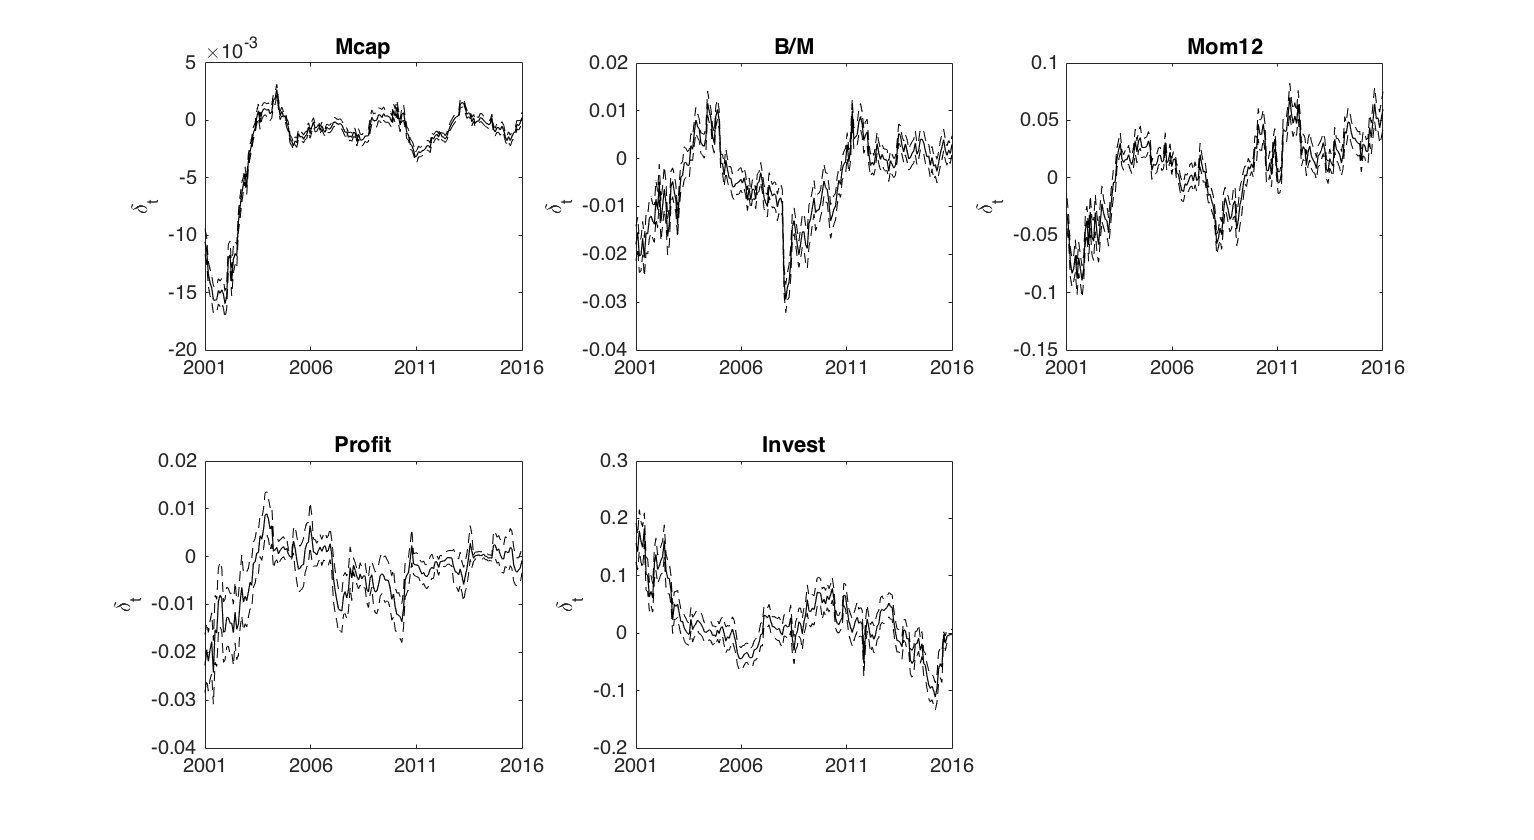
\includegraphics[width=18cm,height=10cm,\textwidth]{pictures/posterior_plots.png}
%   {\captionsetup{justification=centering,singlelinecheck=off}
% \caption{\bfseries Time series plots of the posterior means of the time-varying relation between six-factor alphas and characteristics $\delta_t$}  } 
% \caption*{The figure presents estimation results of the model in Eqs.(\ref{asset}), (\ref{cross}) and (\ref{delta_t}) examining the cross-sectional relation between six-factor alphas and all characteristics simultaneously. In each plot we report posterior results for a given characteristic across our sample period February 2001 to December 2016. The solid line is the posterior mean of $\delta_t$ and the dashed lines represent the 95\% credible interval.}
% \end{figure}
% \end{singlespacing}
% \vspace{-0.45cm}
\par Finally, we examine whether our results are robust to the risk factors included in Eq.(\ref{asset}). In Table \ref{table4} we add the posterior results from the model using alphas from the CAPM, the Fama-French three-factor model, the \citet{carhart1997persistence} four-factor model and the \citet{FAMA20151} five-factor model. The systematic relation between alphas and characteristics are similar across factor models. The posterior means of B/M, Mom12 and Invest vary the most across the factor models, indicating that cross-correlations are the largest between the value, momentum and investment effects, both through the risk factors and the characteristics. Interestingly, we find that the posterior mean of B/M changes sign when the quality factors are considered. The value factor in the three- and four-factor models under-adjusts for the value factor, as alphas are positively related to funds holding value stocks. Conversely, alphas from the five- and six-factor models are positively related to funds holding growth stocks. This contradiction is possibly caused by the interaction between the value factor and the quality factors, which is a negative correlation between the two. All in all, we conclude that the traditional Fama-French risk factors (jointly) insufficiently adjust returns for the main anomalies. 

%  \begin{singlespacing}
%  \begin{table}[h!]
% \small
% \centering
% \setlength{\tabcolsep}{16.5pt}
% {\captionsetup{justification=centering,singlelinecheck=off}
% \caption{\bfseries Multi-factor model alphas vs. characteristics }}
% \caption*{This table presents the results of the estimation of the model in Eqs.(\ref{asset}), (\ref{cross}) and (\ref{delta_t}) based on several Fama-French models. We employ the CAPM, the \citet{fama1993common} three-factor model, the \citet{carhart1997persistence} four-factor model, the \citet{FAMA20151} five-factor model and a six-factor model combining all factors. We estimate the model in each month during the period February 2001 to December 2016, using an estimation period of two years to estimate the factor model in Eq.(\ref{asset}), rolling the window a month at a time. 
%  The characteristics (Z) are the logarithm of market capitalization (Mcap), the logarithm of book-to-market ratio (B/M), the logarithm of one plus the past twelve-month cumulative return (Mom12), operating profitability (Profit) and asset growth (Invest). Each characteristic is standardized by subtracting the cross-sectional mean each month. We report the posterior mean and standard deviation for the aggregate-level parameters in $\bar{\delta}$, based on the posterior distribution of the parameters constructed from 5000 iterations of the Gibbs sampler with the first 2500 iterations discarded as a burn-in period. Estimates in bold font indicates that the 95\% credible interval of the posterior distribution does not include zero. 
% }
% \begin{tabular}{lrrrrr}
% \hline
% \multicolumn{1}{l}{} & \multicolumn{1}{l}{CAPM} & \multicolumn{1}{l}{FF 3FM} & \multicolumn{1}{l}{Carhart 4FM} & \multicolumn{1}{l}{FF 5FM} & \multicolumn{1}{l}{FF 6FM} \\ \hline
% Cnst & 0.000 & \textbf{-0.004}     & \textbf{-0.003}     & \textbf{-0.003}  & \textbf{-0.002} \\ & (0.000) & (0.000)& (0.000) & (0.000) & (0.000) \\ 
% Mcap                 & \textbf{-0.003}          & \textbf{-0.001}                     & \textbf{-0.001}                 & \textbf{-0.002}                     & \textbf{-0.002}                     \\
%                      & (0.000)                   & (0.000)                              & (0.000)                          & (0.000)                              & (0.000)                              \\
% B/M                  & \textbf{0.006}           & \textbf{0.002}                     & \textbf{0.001}                 & \textbf{-0.003}                     & \textbf{-0.003}                     \\
%                      & (0.001)                   & (0.000)                              & (0.000)                          & (0.001)                              & (0.000)                              \\
% Mom12                & \textbf{0.015}           & \textbf{0.008}                      & \textbf{0.004}                  & \textbf{0.007}                      & \textbf{0.005}                      \\
%                      & (0.003)                   & (0.003)                              & (0.003)                         & (0.003)                             & (0.003)                              \\
% Profit               & 0.003                    & 0.001                             & 0.001                          & -0.004                              & -0.003                           \\
%                      & (0.001)                   & (0.001)                              & (0.001)                          & (0.001)                              & (0.002)                              \\
% Invest               & \textbf{-0.046}          & \textbf{-0.023}                     & \textbf{0.020}                  & \textbf{0.014}                      & \textbf{0.017}                      \\
% \multicolumn{1}{l}{} & (0.005)                   & (0.004)                              & (0.004)                          & (0.004)                              & (0.004)                              \\ \hline
% \end{tabular}
% \end{table}
%  \end{singlespacing}

% There are many alternatives to evaluate the performance of mutual funds. A common performance measure is a fund's alpha, the return adjusted for exposures to risk factors that drives most of the fund's return. The typical approach is to regress fund returns onto a set of risk factors. The intercept (alpha) is then interpreted as the abnormal return reflecting the ability of the fund manager. Conventionally, the risk factors are the benchmark portfolio returns of Fama-French, which reflect the main anomalies in the cross-section of returns.  Alternatively, funds are evaluated relative to the characteristic-based benchmark approach of Daniel, Grinblatt, Titman, and Wermers (DGTW; 1997). The DGTW characteristic selectivity (CS) measure controls for the main anomalies by adjusting each fund position relative to the average return of a portfolio holdings stocks with similar characteristics.
% \par Both performance measures stand out for their simplicity, intuitive interpretation and widespread use. The parsimonious structure of both performance measures, however, has it drawbacks. \citet{huij2009use} argue that the Fama-French risk proxies are based on hypothetical stock portfolios that do not incorporate transaction costs, trade impact and trading restrictions, such that the resulting performance estimates for funds may be biased. They propose to use risk factors based on fund returns rather than stock returns to assess fund managerial skill. The DGTW CS measure is based on characteristic-based benchmarks, which are based on coarse quintile sorts to ensure well-populated benchmark portfolios. This might pose a problem when adjusting for multiple anomalies, especially for holdings with extreme characteristics. 
% \par \citet{brennan1998alternative} was the first to look beyond a unilateral explanation of cross-sectional variation in expected returns by either factor betas or characteristics. They find that characteristics (e.g., size, book-to-market, momentum) remain significantly related to expected returns even after the risk-adjustment by a factor model with risk factors based on those same characteristics. In addition, \citet{busse2017double} show that fund-level characteristics yield explanatory power over the cross-section of fund returns after controlling for exposures to the Fama-French risk factors. In Section \ref{section3}, we find that factor betas and fund-level characteristics equally contribute to the explained variation of fund returns. Therefore, we investigate several performance measures which adjusts for both.  

% \subsection{Double-adjusted alpha}
% \label{section4A1}
% For each fund $i$, we estimate the Fama-French six-factor model over a 36-month estimation period, rolling the window a month at a time. This results, given $N_t$ individual funds in month $t$, into a $N_t$ x 1 vector of estimated six-factor alphas $\hat{\alpha}_t$.
% Following \citet{brennan1998alternative}, the estimated alphas constitute the raw material which serves as the dependent variable in monthly cross-sectional regressions\footnote{As opposed to cross-sectional regressions in Section \ref{section3}, the measurement error in the factor betas $\hat{B}$ only effects the dependent variable in Eq.(\ref{double}), and while the factor betas are most probable to be correlated with the characteristics $Z$, there is no a priori reason to expect that the error term $u$ is correlated with the characteristics, such that the estimated coefficients $c$ are unbiased under the null hypothesis. While the EIV-bias is avoided since the estimated betas do not serve as explanatory variables, working with risk-adjusted returns has an important drawback. As noted in \citet{brennan1998alternative}, the risk-adjustment imposes the restriction that the zero-beta rate equals the risk-free rate and the risk premia are constrained to equal the factor means.}
% \begin{equation}
%     \label{double}
%     \hat{\alpha}_{i,t} = c_{0t} + c_{1t}Z_{it-1} + u_i, 
% \end{equation}
% where $Z_{it-1}$ are the lagged fund-level characteristics of fund $i$, $c_{0t}$ measures the average skill across funds in month $t$, $c_{1t}$ measures the rewards of the characteristics with respect to the fund's alpha, and $u_i$ is the idiosyncratic skill of fund $i$. The subscript $t$ for $\hat{\alpha}_{i,t}$ indicates that it is an estimate based on returns up until time $t$. The fund-level characteristics (Z) include the logarithm of market capitalization (Mcap), the logarithm book-to-market ratio (B/M), six-month cumulative return (Mom6), operating profitability (Profit), and investment (Invest). Before including them in the regressions, each characteristic is standardized by subtracting its the cross-sectional mean and dividing by the cross-sectional standard deviation in each month.  
% \par We compute an extended version of the double-adjusted performance measure
% % \footnote{\citet{busse2017double} apply the double-adjusted measure to mutual funds and adjust for size, value, and momentum effects. They propose two different approaches to calculate the double-adjusted measure. Next to the cross-sectional regression approach (used in this paper), they assign funds into portfolios based on a three-way sort on fund-level characteristics, and compare a fund's alpha to the average alpha of the characteristic-based portfolio to which the fund is assigned to. They find that using the portfolio approach does not materially differ the results.} 
% of \citet{busse2017double}. Using the estimated coefficients from Eq.(\ref{double}), the double-adjusted alpha is calculated as 
% \begin{equation}
%     \label{double_alpha} 
%     \alpha^{double}_{i,t} = \hat{\alpha}_{i,t} - c_{1t}Z_{it-1} = c_{0t} + u_i.
% \end{equation} 
% This double-adjusted measure captures performance attributable to fund exposures to risk factors, and also controls for the effects of stocks characteristics, such that we can better capture true fund managerial skill. Beginning with the 36th month during our sample, we compute double-adjusted alphas in each month from the period April 1983 to December 2015, consisting of 393 months. 
% \par Table 4 presents the effects of the adjustment of six-factor alphas for characteristics. Table A2 in the Appendix presents the results using the four-factor model of \citet{carhart1997persistence}. First, we compute average alphas in quintiles sorted on Mcap, B/M, Mom6, Profit or Invest. Each month $t$, we sort funds on lagged characteristics and compute the average alpha for each characteristic quintile. Panel A of Table 4 reports the time series mean of the average six-factor alpha in the characteristic quintiles. The results indicate that for sorts associated with B/M, Mom6 and Invest, the difference between the top quintile and the bottom quintile is statistically significant at the 5\% level. Funds in the top quintile have annualized alphas that are 0.94\% and 1.63\% higher than funds in the bottom quintile for sorts on Mom6 and Invest, respectively, while there is a negative annualized alpha spread of 1.88 for the sort on B/M. There is not a clear pattern across the quintiles sorted on Mcap and Profit. 
% \par Recall that the six-factor model adjust returns for exposures to factors based on Mcap, B/M, Mom6, Profit, and Invest. The results in Panel A of Table 4 suggest that the six-factor model under-adjusts for exposures to the momentum factor, while the model appears to over-adjust for influences related to the value and investment factors. In other words, funds holding high-momentum stocks show higher abnormal return despite the risk-adjustment to the WML factor. Conversely, funds holding positions in high book-to-market and conservative investment stocks under perform, contradictory to previous findings on value and investment effects. Similar conclusions were drawn by \citet{huij2009use}, which find that fund managers following a value-orientated strategy earn a substantially lower premium than those projected by the hypothetical hedge portfolio HML, while the momentum premium earned by funds is larger than that projected by the WML factor.
% \par Furthermore, to provide another indication of the relation between alphas and characteristics, Panel B of Table 4 reports the time-series average of monthly coefficients estimated from Eq.(\ref{double}). We report the average coefficients in univariate regressions with each characteristic and in a joint model. We also calculate \citet{fama1973risk} t-statistics calculated using standard errors with the \citet{newey1986simple} correction of 12 lags\footnote{\citet{petersen2009estimating} has modified the \citet{newey1986simple} correction to accommodate panel data.}. This correction is necessary since the dependent variable in the Fama-MacBeth regressions are derived from overlapping rolling windows. The univariate regressions indicate that there is a statistically significant relation at the 5\% level between alphas and all characteristics except Profit. In a multivariate setting only Invest remains statistically significant. In line with the results of the quintile sorts, the standard factor model benchmark returns for the momentum factor is too low, while the benchmark return is set too high for the value and investment factors. 

% \subsubsection{Double-adjusted DGTW characteristic selectivity measure}
% We extend the characteristic selectivity (CS) measure of  Daniel, Grinblatt, Titman, and Wermers (DGTW; 1997) by also adjusting for profitability and investment effects. We use benchmark returns of portfolio of stocks which is matched to the fund's holdings each quarter along the dimensions of size, value, momentum, profitability, and investment. Specifically, the DGTW CS measure of fund $i$ at time $t$ is calculated as 
% \begin{equation}
%     \label{DGTW_t} 
%     \text{DGTW}_{it} = \sum_{j=1}^{N_{it}} w_{jt-1}(R_{jt}-R^{j}_{t}), 
% \end{equation}
% which is simply the portfolio-weighted average of excess returns over the contemporaneous characteristic-based benchmark portfolio return $R^j_t$ across all holdings $j$ = 1,..., $N_{it}$. Appendix B describes the construction of the benchmark portfolios and how fund holdings are matched to these benchmarks. A DGTW CS value of 0 indicates that the performance of a fund could have been replicated, on average, by simply buying stocks with the characteristics as those held by the fund, and a positive DGTW CS value suggests additional stock-picking skills by the fund's manager. 
% \par Similar to double-adjusted alpha in Section \ref{section4A1}, we conduct an additional adjustment, now for a fund's factor betas. For each fund $i$ in month $t$, we calculate the DGTW CS measure from time $t$-35 until $t$, and calculate the time-series average over this period, which we denote by $\text{DGTW}_{i,t-35:t}$. We estimate the six-factor model over the same period and store the estimated betas $\hat{B}_{it}$. We conduct monthly cross-sectional regressions 
% \begin{equation}
% \label{double1}
%     \text{DGTW}_{i,t-35:t} = c_{0t} + c_{1t}\hat{B}_{it} + u_i,
% \end{equation}
% where $c_{0t}$ measures the average characteristic selectivity skill across funds in month $t$, and $c_{1t}$ measure the rewards of the fund factor betas with respect to the fund's DGTW CS measure, and $u_i$ is the idiosyncratic characteristic selectivity skill of fund $i$. Before including them in the regression, each factor beta is standardized by subtracting its monthly cross-sectional mean. 
% \par Using the estimated coefficients from Eq.(\ref{double1}), we adjust the DGTW CS measure for factor betas as 
% \begin{equation}
%     \label{double_DGTW}
%     \text{DGTW}^*_{i,t-35:t} = \text{DGTW}_{i,t-35:t} - c_{1t}\hat{B}_{it} = c_{0t} + u_i. 
% \end{equation}
% This double-adjusted measure first adjusts performance for stock characteristic effects, and in the second pass regression for exposures to factor betas. If the DGTW CS measure fully adjusts performance for the main anomalies, the factor betas should not convey information about the DGTW CS measure, such that the estimated coefficients $c_{1t}$ are indistinguishable from zero. We compute the double-adjusted DGTW CS measure in each month over from the period April 1983 to December 2015. 
% \par Table 5 presents the effects of the adjustment of the DGTW CS measure for factor betas. Table A3 in the Appendix presents the results when only adjusting for size, value, and momentum effects. First, we compute average DGTW CS measures in quintiles sorted on the six-factor betas, including MKRF (market factor), SMB, HML, WML, RMW, and CMA. Each month $t$, we sort funds on contemporaneous betas and compute the average DGTW CS value for each beta quintile. Panel A of Table 5, reports the time series mean of the average DGTW CS value in the beta quintiles. We find a distinct pattern across quintiles sorted on the SMB and WML betas, as the average DGTW CS measure increases nearly monotonically across the SMB and WML quintiles and indicates a sizable spread of 0.057 (t = 2.32) and 0.124 (t = 6.71) between the top and bottom quintiles of SMB and WML, respectively. Regarding quintiles sorted on HML, RMW, or CMA, the top-minus-bottom DGTW CS measures are, on average, indistinguishable from zero. 
% \par Panel B of Table 5 reports the time-series average of monthly coefficients estimated from Eq.(\ref{double1}), with \citet{fama1973risk} t-statistics calculated using standard errors with the \citet{newey1986simple} correction of 12 lags. Again, we find that SMB and WML betas are significantly related to the cross-section of DGTW CS measures, suggesting that the characteristic-based benchmark approach under-adjusts for size and momentum effects. We find statistical insignificant coefficients for the HML, RMW, and CMA betas, indicating that exposures to the value, profitability, and investment factors do not convey new information after the characteristic-based adjustment. 

% \subsection{Bayesian alphas }
% We employ the hybrid approach of \citet{cosemans2015estimating} for estimating factor betas that incorporate fund-level characteristics as prior information. This method relates to the asset pricing literature which condition factor betas on firm fundamentals and economic state variables. Previous literature including the works of \citet{lewellen2010skeptical}, \citet{avramov2006asset}, \citet{chordia2012cross} provide empirical evidence that factor betas are related to firm characteristics such as market capitalization and book-to-market ratios. By incorporating cross-sectional information on factor betas we may increase the accuracy of sample estimates since factor betas might be similar across funds with overlapping holdings. For illustration, consider we estimate a momentum beta of 0.1 for a fund with limited return data. However, based on the funds with similar holdings we find that momentum betas are normally distributed with moments equal to 0.2 and 0.4. Based on this information the sample estimate of 0.1 might be biased downwards.
% \par For each fund $i$, we conduct rolling-window estimations (window size of $\tau$ = 36 months) of the Fama-French six-factor model  

% \begin{equation}
%     \label{factor_model6}
%     R_{it} = \alpha_i + \beta_{i1}F_{1t} + ... + \beta_{i6}F_{6t} + \epsilon_{it} = \alpha_{i,t} + \beta'_{i,t} F_t + \epsilon_{it}, \hspace{0.2cm} t = t-\tau,...,t,
% \end{equation}
% where $R_{it}$ denotes excess monthly returns of fund $i$ and $F_t$ = [$F_{1t}$,...,$F_{6t}$] are the six-factor benchmark returns in month $t$, and $\epsilon_{it}$ is the residual return which is normally distributed with zero mean and variance $\sigma^2_{i,t}$. The subscript $t$ for $\alpha_{i,t}$ and $\beta_{i,t}$ indicates that we use monthly returns up until time $t$. To incorporate the fund-level characteristics as prior information, we use Bayesian techniques to estimate Eq.(\ref{factor_model6}). In the spirit of \citet{cosemans2015estimating}, we specify diffuse priors for alpha and the idiosyncratic variance $\sigma^2_{i,t}$ and assume a normal distribution for the prior of $\beta_{i,t}$, that is, 
% \begin{equation}
% \label{prior_beta}
%     p(\alpha_{i,t}) \propto 1, \hspace{0.2cm} p(\sigma^2_{i,t})  \propto \sigma^{-2}_{i,t} \hspace{0.2cm} \text{and} \  \hspace{0.2cm} \beta_{i,t} \sim \mathcal{N}(\bar{\beta}_{i,t},\Sigma_{\beta_{i,t}}). 
% \end{equation}
% The prior specification is unique to each fund for each month by including fund-specific information on the fund's holdings. In the next section we elaborate on how we determine the parameters in the prior of $\beta_{i,t}$. 
% \par We estimate the factor model using the Markov Chain Monte Carlo (MCMC) Gibbs sampler\footnote{Examples of Bayesian inference in asset pricing models are presented in \citet{mcculloch1990posterior} and \citet{harvey1990bayesian}. For an extensive reading on the application of the Gibbs sampler in econometrics, we refer to \citet{de2006gibbs}}. An attractive feature of MCMC techniques is that samples of random drawings can be generated from the joint posterior  indirectly, without the need to specify the exact form of this joint distribution directly. The Gibbs sampler uses an iterative procedure to create Markov chains by simulating from full conditional posteriors instead which are typically much easier to derive. After the Markov chains have converged, the sets of draws that are obtained from the conditional posteriors can be effectively considered as samples from the joint posterior. We describe the steps in the Gibbs sampler thoroughly in Appendix C. We use the posterior mean of $\alpha_{i,t}$ as our (double-adjusted) performance measure, which we denote as $\alpha^{Bayes}_{i,t}$.

% \subsubsection*{Prior estimation}
% We specify a monthly panel model to elicit a prior for factor betas of fund $i$ in month $t$, 
% \begin{equation}
% \label{panel1}
%     R_{it} = \alpha^*_i + \beta^*'_{i,t|t-1}F_t + \eta_{it}, 
% \end{equation}
% which is the same model as in Eq.(\ref{factor_model6}), but now using the entire panel rather than fund-specific over rolling windows. The idiosyncratic return $\eta_{it}$ is normally distributed with zero mean and variance $\sigma^2_{\eta_i}$ and is assumed to be independent across funds. We define prior beta as follows
% \begin{equation}
% \label{con_beta}
%     \beta^*_{i,t|t-1} = \delta_i + \xi' Z_{it-1}, 
% \end{equation}
% where each factor beta is parameterized as a linear function of lagged fund-level characteristics (Z). The fund-level characteristics (Z) include the logarithm of market capitalization (Mcap), the logarithm book-to-market ratio (B/M), six-month cumulative return (Mom6), operating profitability (Profit), and investment (Invest). Before including them in the regressions, each characteristic is standardized by subtracting its the cross-sectional mean and dividing by the cross-sectional standard deviation in each month. 
% \par In the panel model the regression constant $\delta_i$ = [$\delta_{i1},...,\delta_{i6}$]' is unique to each fund, while the loadings on the characteristics are pooled in $\xi$ = [$\xi_1$,...,$\xi_6$]. The fund-specific parameters mitigates the omitted variable bias by accounting for effects on beta which are constant but vary across funds. The pooled parameters increase estimation precision by using cross-sectional information from the entire sample, as we expect there exists a generic relation between factor betas and characteristics across funds. 
% \par Given the specification of the prior beta, substitution of Eq.(\ref{con_beta}) in Eq.(\ref{panel1}) and some rewriting yields
% \begin{equation}
% \label{panel}
%     R_{it} = \alpha^*_i + (\delta_{i1} + \xi_1'Z_{it-1})F_{1t} + ... + (\delta_{i6} + \xi_6'Z_{it-1})F_{6t} + \eta_{it}.
% \end{equation}
% We use the MCMC Gibbs sampler to estimate Eq.(\ref{panel}), as this Bayesian approach allows let some parameters vary across funds to capture unobserved heterogeneity in factor betas, while pooling other parameters to exploit cross-sectional information.  Using the estimates from the panel model we can compute posterior results for $\beta^*_{i,t|t-1}$, which constitute the prior mean and variance for $\beta_{i,t}$ in Eq.(\ref{prior_beta}). We describe the steps in the Gibbs sampler thoroughly in Appendix D.

% \subsection{Importance of adjustment for characteristics}
% \label{importance}
% To provide initial evidence that the standard factor model alpha imperfectly controls for passive loadings on characteristics, we examine the Fama-French six-factor alpha of funds sorted into quintiles based on the fund-level market capitalization, book-to-market ratio, past twelve-month cumulative return, operating profitability, and investment. During the sample period April 1983 to December 2015, we estimate each month the six-factor model alpha over the past 36 months. We then funds into deciles based on fund-level characteristics averaged over the past 36-month window, lagged one month, and we compute the average standard alpha in each characteristic decile. 
% \par Table 4 reports the average six-factor alpha in the characteristic decile. The results indicate that for sorts associated with B/M, Mom6 and Invest, the difference between the top decile and the bottom decile is statistically significant at the 5\% level. Funds in the top decile have annualized alphas that are 1.20\% and 1.17\% higher than funds in the bottom decile for sorts on Mom6 and Invest, respectively, while there is a negative annualized alpha spread of 1.31\% for the sort on B/M. There is not a clear pattern across the deciles sorted on Mcap and Profit. 
%  \par Recall that the six-factor model adjusts returns for exposures to factors based on Mcap, B/M, Mom6, Profit, and Invest. The results in Table 4 suggest that the six-factor model under-adjusts for exposures to the momentum factor, while the model appears to over-adjust for influences related to the value and investment factors. In other words, funds holding high-momentum stocks show higher abnormal return despite the risk-adjustment to the WML factor. Conversely, funds holding positions in high book-to-market and conservative investment stocks under perform, contradictory to previous findings on value and investment effects. Similar conclusions were drawn by \citet{huij2009use}, which find that fund managers following a value-orientated strategy earn a substantially lower premium than those projected by the hypothetical hedge portfolio HML, while the momentum premium earned by funds is larger than that projected by the WML factor.
%  \par Furthermore, Table 5 reports the estimated loadings on characteristics from the panel regression model in  Eq.(\ref{double_alpha}). We compute the average regression coefficients across all sample months. We also calculate \citet{fama1973risk} t-statistics calculated using standard errors with the \citet{newey1986simple} correction of 12 lags.\footnote{\citet{petersen2009estimating} has modified the \citet{newey1986simple} correction to accommodate panel data.} This correction is necessary since there is overlap in the estimation windows. The results in Table 5 show that, on average, fund returns are sensitive to the characteristics of the stocks held in fund portfolios. All characteristics but Invest yield a statistically significant relation at the 5\% level with fund returns. 
 
%  \subsection{Effects of double adjustment}
%  The results in Section \ref{results} demonstrate that the characteristics of the holdings of funds are an important determinant of expected fund returns. In Section \ref{importance} we have demonstrated an important shortcoming of the standard factor models, insofar as they attribute skill to passive exposures to characteristics. We have proposed a new performance measure which accounts for the performance attributable to characteristics to produce a purer quantification of skill. In this section we investigate whether our double-adjusted performance measure adequately adjusts performance to characteristics. We also examine whether our performance measure materially impacts fund percentile performance rankings relative to using the standard factor model alpha. 
%  \par Similar to the previous section, we sort funds into deciles based on  fund-level characteristics averaged over the past 36-month period, lagged one month. For each month in our sample we compute the average double-adjusted performance measure for each characteristic decile. Table 6 shows that the top-minus-bottom spread in alpha is statistically indistinguishable from zero for each characteristic sort. For the sorts on B/M and Mom12 we still find a similar pattern in double-adjusted alpha as with standard alpha, but the characteristic-adjustment seems to have mitigated these patters. Thus, the new performance measure is less sensitive to passive loadings on characteristics, such that performance attributable to characteristics is mostly removed from our double-adjusted alpha. 
%  \par One might anticipate that the new performance measure could alter the performance ranking of funds. In each month in our sample, we sort funds into percentiles based on double-adjusted alpha and on standard six-factor alpha. Table 7 presents the distribution of the difference in percentile rankings. When we compare percentile performance rankings between the two performance measures, we find that the median change in percentile rankings is 8.67\%. Moreover, many funds exhibit dramatic changes in performance rank, with 25 (10) of funds experiencing a mean change in percentile ranking of at least 16.25\% (25.47\%). 
 
% \subsection{Effects of adjustment alpha for characteristics}
% The results in Section \ref{section4b} indicate that the standard factor models provide inadequate risk-adjustments to the common risk factors. As a consequence, alpha does not fully reflect performance in excess of risk factors as it attributes skill to passive exposure to characteristics underlying these factors. Double-adjusted alpha rectifies this by providing a performance measure corrected for exposures to both risk factors and underlying characteristics. First, we investigate whether the adjustment for characteristics materially differs the performance ranking of funds. Second, we conduct a battery of simulations to examine whether the double-adjusted performance measure is better at identifying stock-picking skill. 
% \par 
% Specifically, we rank funds each month in percentiles according to their alphas and double-adjusted alphas, and compare the differences between the performance percentile rankings. Figure 1 shows the absolute differences between performance percentile rankings caused by adjusting alpha for characteristics. Funds experience a median change in percentile rank of about five percent when adjusting alpha. That is, a fund that ranks in the 50th percentile based on alpha ranks in the 45th or 55th percentile with the characteristics adjustment. Moreover, we find that 25 percent of funds experience a change in percentile ranking of at least 10 percent.
% \subsubsection*{Simulations}
% For the simulations, we follow the framework set by \citet{busse2017double}. The goal of the simulations is to assess whether the performance measures can distinguish skill from luck. We simulate fund returns with zero stock-picking skills by design and compute the standard factor alpha and the double-adjusted alpha. The superior performance measure identifies no skill across simulated funds, which should result in marginal cross-sectional differences in alpha. The bootstrap simulations of \citet{busse2017double} are similar to the simulations in \citet{kosowski2006can} and \citet{fama2010luck}, which investigate skill in the cross-section of fund returns. 
% \par 
% We simulate funds returns by repeatedly constructing a fund's portfolio by sampling stocks from the actual data. For each fund in the sample, we create a simulated fund portfolio with holdings similar to the actual fund's portfolio, in terms of the fund's TNA, number of holdings, portfolio weights and the characteristics of each holding. First, each month we sort the funds in the actual sample into quintiles based on funds' TNA. Within each fund size group, we record all the unique stocks held by all funds, and we assign each stock into quintiles for each stock characteristic. 
% \par 
% We simulate a fund's portfolio as follows. For each fund at a given report date, we randomly select a stock for each position in the fund's portfolio from a list of stocks matching the fund's size ranking. We further narrow down the list of stocks to those matching the  quintile rankings of the given position. To the stocks in the final list we assign sampling probabilities equal to the number of funds holding each stock. The number of shares held of a simulated position equals the initial investment of the original position divided by the price of the simulated position at the report date. We maintain this simulated portfolio in subsequent months up until the next report date with a maximum holding period of three months. We compute a fund's portfolio-weighted gross return using portfolio weights based on the number of shares (determined at the report date) and the returns (from the actual data) of the simulated stocks\footnote{Fund returns in the CRSP Mutual Fund Database are reported net of all operating expenses (expense ratio). \citet{carhart1997persistence} show that expense ratios are negatively related with net returns. \citet{wermers2000mutual} use fund holdings to decompose gross fund returns into several components and show that stock-picking skills of fund managers are masked by expense ratios. By using gross returns derived from the fund's holdings in the simulations, we can better measure skill across funds.  }. 